\section{Mixture Models}

In this question we get introduced to mixture models.
\subsection{Introduction to Mixture Models}
In your own words, explain how the MM algorithm can deal with non convex optimization objective functions by considering simpler convex objective functions.
\begin{qsolve}
    \begin{qsolve}[]
        the MM algorithm can deal with non convex optimization objective functions by considering simpler convex objective functions by using the Expectation-Maximization (EM) algorithm. 
        in this algorithm we define a simpler function like $g(\theta)$ and we try to maximize it so if we maximize this function the $\bar{\theta}$ is actually the maximizer of the original non-convex function $f(\theta$).
        
        the function we define as $g(\theta)$ is a lower bound of the original function $f(\theta)$ like solving a dual problem in optimization.this works as the equation below:
        $$f(\theta) \geq g(\theta) \quad \forall \theta$$
        $$ \text{if}\ \theta = \bar{\theta} \text{ then } f(\bar{\theta}) = g(\bar{\theta})$$
    \end{qsolve}
\end{qsolve}
\subsection{Mixture Models for specific distribution}
You are given a data set $D = \{(x_1, y_1), \ldots, (x_N, y_N)\}$, $x_i \in \mathbb{R}^d, y_i \in \mathbb{R}, i = 1, \ldots, N$. The data points accumulate on $m$ different lines, $a_j^Tx_i = y_i$, for $a_j \in \mathbb{R}^d, j = 1, \ldots, m$.

\begin{figure}[h]
    \centering
    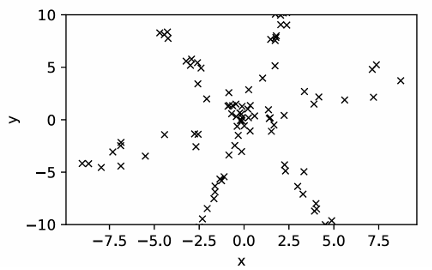
\includegraphics[width=0.5\textwidth]{image.png}
    \caption{d=1 and m=3}
\end{figure}

Then
\[
p(x, y \mid \theta) = \sum_{j=1}^{m} \pi_j \frac{1}{\sqrt{2\pi\sigma^2}} \exp \left( -\frac{\left( a_j^T x - y \right)^2}{2\sigma^2} \right),
\]
where $\theta = (\pi_{1:m}, a_{1:m})$, $\sum \pi_j = 1$, $\pi_j \ge 0$ and $\sigma > 0$ is given and fixed.

\begin{itemize}
    \item Find the responsibilities in the E-step of Soft EM,
    \[
    r_{nk}^{(t)} = p \left( z_n = k \mid x_n, y_n, \theta^{(t-1)} \right).
    \]
    
    \item Write down the class predictions $z_n^{(t)}$ for $(x_n, z_n)$ in the E-step of Hard EM in terms of $r_{nk}^{(t)}$.
    
    \item Assume that we observe the true labels $z_1, \ldots, z_\ell$ for the first $\ell$ datapoints, $\ell < N$. How can we modify the E-step of Soft EM to incorporate the additional information?
\end{itemize}
\begin{qsolve}
    \begin{qsolve}[]
        we know that:
        $$p(z_n=k|x_n,y_n,\theta) = \frac{p(x_n,y_n|z_n=k,\theta)p(z_n=k|\theta)}{\sum_{j=1}^{m}p(x_n,y_n|z_n=j,\theta)p(z_n=j|\theta)}$$
        we define $p(z_n=j,\theta)$ as $\pi_j$ and from the given information $r_{nk}^{(t)} = p \left( z_n = k \mid x_n, y_n, \theta^{(t-1)} \right)$ so we can wtirite:
        $$p(x,y|z=k) = \frac{1}{\sqrt{2\pi\sigma^2}} \exp \left( -\frac{\left( a_k^T x - y \right)^2}{2\sigma^2} \right)$$
        $$\Rightarrow r_{nk}^{(t)} = \frac{\pi_k^{(t-1)}\exp \left( -\frac{\left( a_k^T x_n - y_n \right)^2}{2\sigma^2} \right)}{\sum_{j=1}^{m}\pi_j^{(t-1)}\exp \left( -\frac{\left( a_j^T x_n - y_n \right)^2}{2\sigma^2} \right)}$$
        for the second part we have:
        $$z_n^{(t)} = \arg \max_{k} \log r_{nk}^{(t)}$$
        we calculated the $r_{nk}^{(t)}$ in the previous part so we can write:
        $$z_n^{(t)} = \arg \max_{k} \log r_{nk}^{(t)} = \arg \max_{k} \log \left( \frac{\pi_k^{(t-1)}\exp \left( -\frac{\left( a_k^T x_n - y_n \right)^2}{2\sigma^2} \right)}{\sum_{j=1}^{m}\pi_j^{(t-1)}\exp \left( -\frac{\left( a_j^T x_n - y_n \right)^2}{2\sigma^2} \right)} \right)$$
        the dominator is the same for all $k$ so we can ignore it and we can write:
        $$z_n^{(t)} = \arg \max_{k} \log \pi_k^{(t-1)} - \frac{\left( a_k^T x_n - y_n \right)^2}{2\sigma^2}$$
        
        and for the third part we can use the true labels to modify the E-step of Soft EM by setting the $r_{nk}^{(t)}$ to 1 for the true label and 0 for the others. so the new $r_{nk}^{(t)}$ will be:
        \splitqsolve[\splitqsolve]
        for the labeled data:
        $$r_{nk}^{(t)} = \begin{cases} 1 & \text{if } z_n = k \\ 0 & \text{otherwise} \end{cases}$$
        for the unlabeled data:
        $$r_{nk}^{(t)} = \frac{\pi_k^{(t-1)}\exp \left( -\frac{\left( a_k^T x_n - y_n \right)^2}{2\sigma^2} \right)}{\sum_{j=1}^{m}\pi_j^{(t-1)}\exp \left( -\frac{\left( a_j^T x_n - y_n \right)^2}{2\sigma^2} \right)}$$
    \end{qsolve}
\end{qsolve}